%Encabezado estándar
\documentclass[10pt,a4paper]{article}
\usepackage{pgfplots}
\usepackage[utf8]{inputenc}
\usepackage{amsmath}
\usepackage{multirow}
\usepackage{amssymb}
\usepackage{amsthm}
\usepackage{hyperref}
\usepackage{graphicx}
\usepackage{subfigure} %paquete para poder añadir subfiguras a una figura
\usepackage{listings}
\usepackage{color}
\usepackage{float}
\usepackage[toc,page]{appendix} %paquete para hacer apéndices
\usepackage{cite} %paquete para que Latex contraiga las referencias [1-4] en lugar de [1][2][3][4]
\usepackage[nonumberlist]{glossaries} %[toc,style=altlistgroup,hyperfirst=false] 
%usar makeglossaries grafo para recompilar el archivo donde están los grafos y que así salga actualizado
\author{Gustavo Rivas Gervilla DNI: 75570417F \\ gustavofox92@correo.ugr.es \\5º Doble Grado en Ing. Informática y Matemáticas \\Grupo 3}
\title{Práctica 3.b: Algoritmos Genéticos para el Problema de la Selección de Características \\ AGG \\ AGE}
\date{}

\addtolength{\oddsidemargin}{-.875in}
\addtolength{\evensidemargin}{-.875in}
\addtolength{\textwidth}{1.55in}
%Configuración especial
\setlength{\parindent}{0cm}
\pretolerance=10000
\tolerance=10000
\renewcommand{\contentsname}{\color[rgb]{0.0,0.0,0.21}Índice}
\renewcommand{\tablename}{\color[rgb]{0.5,0.0,0.0}Tabla}

\hypersetup{
  colorlinks=true,%colorear el texto en lugar de poner una caja de color alrededor
  citecolor=orange,%citas bibliográficas, del estilo [8]
  urlcolor=orange,%urls
  linkcolor=[rgb]{0.0,0.0,0.21}}%links internos como los del índice
  
\lstdefinestyle{customPy}{
  belowcaptionskip=1\baselineskip,
  breaklines=true,
  frame=L,
  xleftmargin=\parindent,
  language=Python,
  showstringspaces=true,
  basicstyle=\footnotesize\ttfamily,
  keywordstyle=\bfseries\color{green!40!black},
  commentstyle=\itshape\color{purple!40!black},
  identifierstyle=\color{blue},
  stringstyle=\color{orange},
}

\begin{document}
\lstset{language=Python, style=customPy}
\maketitle

\newpage

\tableofcontents

\newpage

\section{\color[rgb]{0.0,0.0,0.21}Descripción/formulación del problema abordado}
Lo que intentamos hacer con nuestros algoritmos es encontrar un conjunto de características de unos datos que nos permitan realizar una clasificación suficientemente buena de nuevos datos que nos lleguen con las mismas características.\\

Hay un problema muy habitual en la vida real y es la de clasificar una serie de elementos en distintas categorías en función de información sobre ellos, esta tarea puede ser realizada por personas o, lo que es más eficiente, por un ordenador. Para realizar tal clasificación es habitual que se recojan multitud de datos sobre los distintos elementos que se quieren clasificar, de modo que en base a esta información podamos decidir si el elemento es de una categoría o de otra. Pensemos por ejemplo en clasificar fruta en base a si se desecha o no. Podemos pensar en recoger datos sobre el tamaño de esa fruta, su color, su textura o su dureza y en base a estas mediciones una máquina debería clasificar la fruta en buena o mala.\\

El problema está en que normalmente no se conoce tan bien el campo de estudio como para saber a ciencia cierta qué datos recoger, qué datos serán más relevantes a la hora de clasificar elementos de una determinada población. Entonces lo que se hace es recoger gran cantidad de información sobre los elementos para al menos intentar que no haya carencias en la información, esto por supuesto conlleva tanto el coste de adquirir esa información (no sabemos cómo de caro es realizar una determinada medición) como el coste computacional de procesar toda esa información. Entonces lo que nos gustaría es averiguar qué información, de entre toda la que hemos obtenido, es la verdaderamente relevante para la clasificación que queremos realizar.\\

Entonces partiendo de un conjunto de datos de aprendizaje, valores de características de distintos elementos, queremos ver con qué subconjunto de características podemos hacer una buena clasificación de esos elementos, así si tenemos que cada dato viene dado por una lista de n características $[f_1, f_2, ..., f_n]$ queremos obtener un subconjunto de esas características, de modo que teniendo sólo la información $[f_{s1}, ..., f_{sm}]$, se haga una buena clasificación del conjunto de datos de aprendizaje, del que conocemos por supuesto la clasificación perfecta de dichos datos. Y esperamos que con esa misma información se clasifiquen lo mejor posible nuevos elementos de fuera de la muestra de aprendizaje.\\

\newpage

\section{\color[rgb]{0.0,0.0,0.21}Descripción de la aplicación de los algoritmos empleados al problema}

Dado que estamos ante un problema de selección las soluciones se representarán como vectores binarios de booleanos de tamaño el número de características a elegir, indicando si una característica se considera o no, así tendremos claramente un espacio de búsqueda de $2^n$, siendo $n$ el número de características a elegir que también lo podemos ver como el tamaño del problema abordado.\\

Entonces para evaluar como de buena es una determinada solución hacemos lo siguiente:\\

\begin{lstlisting}
tomamos de cada dato de entrenamiento las caracteristicas seleccionada por la solucion.

for cada dato de entrenamiento:
	clasificador_dato = construir clasificador 3NN con el resto de datos
	ver si clasificador_dato clasifica correctamente a ese dato
	
return porcentaje de aciertos
\end{lstlisting}

Nuestros algoritmos irán explorando, según su mecanismo, el espacio de soluciones empleando la función anterior para tomar decisiones sobre qué movimientos se realizan en dicho espacio de búsqueda. Para poder generar las soluciones vecinas a una dada empleamos el operador de Flip, el cual funciona del siguiente modo:\\

\begin{lstlisting}
def flip(sol, idx):
	cambiar el valor de la pos. idx de la sol por su negado
\end{lstlisting}

Cuando finalice su proceso de búsqueda los algoritmos nos devolverán la solución que ellos han elegido (junto con el score dentro de la muestra de entrenamiento calculada como hemos dicho antes). Entonces una vez tenemos la solución nos queda por evaluar cómo de bien se clasifican los datos empleando un clasificador 3NN construido sólo con aquellas características seleccionadas por nuestra solución:\\

\begin{lstlisting}
claficador = construir clasificador con los datos de entrenamiento solo con las caracterisiticas seleccionadas por nuestra solucion
return el porcentaje de acierto de este clasificador etiquetando los datos de test de los que consideramos solo las caracteristicas seleccionadas por la solucion
\end{lstlisting}

A cada algoritmo le daremos solamente los datos de entrenamiento separados en características y etiquetas pera que con la estragia de búsqueda que implemente nos devuelva la mejor solución posible para él, luego la evaluación de la solución final la haremos fuera del algoritmo con los datos de test (en la sección 8 explicaremos cómo hemos generado las particiones). Para aquellos algoritmos que empleando algún tipo de aleatoriedad en sus decisiones inicilizaremos la semilla aleatoria antes de la ejecución de dicho algoritmo.\\

Para generar las soluciones aleatorias lo que hacemos al inicio de cada algoritmo es:\\

\begin{lstlisting}
p_inicial = vector[30][num_caracteristicas]

for cada p in p_inicial:
	p = vector de num_caracteristicas valores booleanos aleatorios
\end{lstlisting}

El mecanismo de selección que utilizamos es el de torneo binario que consiste en lo siguiente:\\

\begin{lstlisting}
for 30 o 2 veces(segun estemos en AGG o AGE):
	padre1 = individuo aleatorio de la poblacion actual
	padre2 = individuo aleatorio de la poblacion actual
	seleccionamos el mejor entre padre1 y padre2 segun su score
	almacenamos el elegido en un vector de padres elegidos
\end{lstlisting}

El operador de cruce que emplearemos es el HUX ya que como se dijo en clase funciona mejor que el que se explica en las transparencias (mi compañero Jacinto Carrasco Castillo ha probado ambos operadores obteniendo efectivamente mejores resultados con este operador de cruce) y funciona así:\\

\begin{lstlisting}
def cruce(padre1, padre2):
	creamos dos nuevos individuos hijo1 e hijo2
	copiamos en los hijos aquellos genes que son iguales en ambos padres
	
	for gen in los genes que difieren en los padres:
		hijo1[gen] = valor booelano aleatorio
		hijo2[gen] = not hijo1[gen]
		
	return los hijos		
\end{lstlisting}

El operador de mutación es el \textit{flip} que hemos usado para la generación de vecinos, al cuál le damos el individuo a mutar y el gen a cambiar de valor.\\

\newpage

\section{\color[rgb]{0.0,0.0,0.21}Descripción en pseudocódigo de los algoritmos}
\subsection{\color[rgb]{0.0,0.0,0.51}AGG (AGG.py)}

\begin{lstlisting}
padres = poblacion inicial de 30 individuos aleatoria
ordenamos los padres de peor a mejor segun score

while n_evals < max_evals:
	#seleccion
	padres_seleccionados = seleccionamos 30 padres por torneo binario (con repeticion)
	
	#cruce
	cruzamos las primeras n_cruces parejas de padres_seleccionados y metemos el resultado en hijos
	
	aniadimos a hijos copias de los padres que no se han cruzado
	
	#mutacion
	seleccionamos n_mutaciones hijos aleatoriamente para mutar (con repeticion)
	seleccionamos n_mutaciones genes a mutar (con repeticion)
	
	for cada par (hijo,gen) seleccionado:
		modificamos el gen de ese hijo por su complementario
		
	#remplazamiento
	if mejor_hijo es peor que mejor_padre:
		peor_hijo = mejor_padre
		
	padres = hijos
	ordenamos padres
	
return mejor padre de la poblacion actual		
\end{lstlisting}

\newpage

\subsection{\color[rgb]{0.0,0.0,0.51}AGE (AGE.py)}

\begin{lstlisting}
umbral = 2 * n_caracteristicas / 1000 #para mutacion

padres = poblacion inicial de 30 individuos aleatoria
ordenamos los padres de peor a mejor segun score

while n_evals < max_evals:
	#seleccion
	padre1 = padre elegido por torneo binario
	padre2 = padre elegido por torneo binario
	
	#cruce
	hijo1, hijo2 = resultado de cruzar los dos padres
	
	#mutacion
	if num aleatorio en el [0,1] <= umbral:
		mutamos un gen aleatorio de uno de los dos hijos elegido aleatoriamente
		
	#remplazamiento
	if mejor hijo es mejor que el penultimo padre:
		antepenultimo padre = mejor hijo
		
		if el otro hijo mejor que el peor padre:
			peor padre = el otro hijo
	elif mejor hijo mejor que peor padre:
		peor padre = mejor hijo
		
	ordenamos los padres
	
return mejor padre en la poblacion actual
\end{lstlisting}

\newpage

\section{\color[rgb]{0.0,0.0,0.21}Breve descripción del algoritmo de comparación}

Para el algoritmo de comparación, SFS, lo que hacemos es lo que vamos a reflejar en el siguiente pseudocódigo, la principal diferencia es que no tenemos la función usual flip sino que hemos hecho una función especial para poder realizar una función vectorizada en Python (aunque no produce ninguna mejora en tiempo a la versión que tendríamos si simplemente tuviésemos un for que recorriese las características que quedan por añadir hasta encontra la de mayor ganancia), esta función crea una nueva solución poniendo a True una componente de la solución que le pasamos y nos da su porcentaje de clasificación, como hacemos en el resto de algoritmos. Dicho esto pasamos al pseudocódigo:

\begin{lstlisting}
sol = un array binario con todo False #conjunto vacio de caracteristicas

while tengamos ganancia and queden caracteristicas por aniadir:
	calcular el score de cada caracteristica por aniadir al agregarla al conjunto actual
	tomar la caracteristica que de mejor score en el calculo anterior
	
	if el score aniadiendola es mejor que el de el conjunto mejor al que habia:
		se agrega dicha caracteristica al conjunto
		quitamos esa caracteristica de el conjunto de caracteristicas por aniadir
	else:
		no tenemos ganancia y acabamos el bucle
		
return el conjunto de caracteristicas al que hemos llegado
\end{lstlisting}
\newpage

\section{\color[rgb]{0.0,0.0,0.21}Procedimiento considerado para desarrollar la práctica}

\subsection{\color[rgb]{0.0,0.0,0.51}Desarrollo}

El código usado en prácticas lo he implementado yo a partir de las explicaciones dadas tanto en clase de prácticas como de teoría sobre los distintos algoritmos, siendo de mucha utilidad las indicaciones del gruión de práctias y del seminario.\\

La parte que no ha sido implementada por mí es la correspondiente a la evaluación de las soluciones, es decir, tanto el KNN como los mecanismos de evaluación de las soluciones. Para ello he usado el código desarrollado por \textbf{Alejandro García Montoro} el cuál ha implementado tanto el clasificador KNN como los mecanismos para obtener el score de las soluciones dentro (con LOO) y fuera de la muestra con PyCUDA que permite insertar código CUDA en código Python. Con lo cual los tiempos de ejecución bajan considerablemente con respecto a los tiempos de la práctica anterior ya que el cuello de botella de los algoritmos, que es la evaluación de las soluciones con LOO, se ejecuta en la tarjeta gráfica, siendo mucho más rápidos los cálculos.\\

\subsection{\color[rgb]{0.0,0.0,0.51}Manual de usuario}
Los algoritmos han sido implementados en Python 3.5.1 para su ejecución son necesarios tener instalados los módulos compatibles con esta versión de Python siguientes:\\

\begin{itemize}
\item numpy (v 1.8.2) \textbf{sudo apt-get install python-numpy}
\item scikit \textbf{sudo apt-get install python-scikits-learn}
\item jinja2
\item pycuda
\item El resto de módulos empleados suelen venir con las distribuciones básicas de Python (random, sys y time).
\end{itemize}

Cada uno de los algoritmos están implementados en distintos ficheros de los que podemos ver su contenido en el \textbf{\textcolor{green}{LEEME}} que se nos pide que incluyamos con el código. Los experimentos han sido ejecutados usando el fichero main al que le pasamos por argumentos el nombre del algoritmo a usar: 3NN, SFS, AGG o AGE. La semilla se establece dentro del fichero al inicio de la ejecución del algoritmo para cada una de las particiones. Esto lo hemos hecho así para poder cortar la obtención de datos cuando sea necesaria y poder retomar los experimento desde la partición por las que nos quedáramos, así no se desajusta la semilla con la que hacemos los experimentos al retomar.\\

Entonces para ejecutar por ejemplo los experimentos para el AGG lo que haremos es \textit{python mainCUDA.py AGG} y se ejecutará el algoritmo sobre todas las particiones de datos que tenemos.\\

En el directorio \textbf{\textcolor{green}{make\_partitions32b}} tenemos tanto los archivos arff como los códigos necesarios para elaborar las particiones que serán utilizadas por nuestros algoritmos. Esto no es necesario para ejecutar los programas puesto que en el directorio \textbf{\textcolor{green}{partitions32b}} tenemos almacenadas todas las particiones construidas. No obstante si se quisiera replicar el procedimiento de desarrollo de particiones lo que haríamos sería: eliminar los archivos con extensión .npy del directorio \textbf{make\_partitions32b} (para tener seguridad de que no se corrompan dichos archivos), ejecutar el loader con la instrucción \textbf{python loader.py} y a continuación elaborar las particiones con \textbf{python partition\_maker.py} (dentro de este directorio que es donde se encuentran ambos códigos). Esto generará diversos archivos de extensión .npy con nombres que empiezan por arr, wdbc o libras (según la base) seguida de un número y la palabra test o training.\\

Estos archivos deberán reemplazar a aquellos que se encuentran en el directorio \textbf{partitions32b} y ya podremos ejecutar los algoritmos con dichas particiones desde el main.\\

\newpage
\section{\color[rgb]{0.0,0.0,0.21}Experimentos y análisis de resultados}

\subsection{\color[rgb]{0.0,0.0,0.51}Descripción de los casos del problema empleados y de los valores de los parámetros}


Estás prácticas han sido implementadas en Python 3.5.1 y ejecutadas sobre un ordenador son S.O. Arch Linux, de 12GB de RAM y procesador Intel Core i7 930 2.80GHz y tarjeta gráfica NVIDIA GeForce GTX 780. Este ordenador pertenece a Alejandro Garcia Montoro ya que tuve problemas al intentar usar los drivers oficiales de Nvidia en Ubuntu (necesarios para ejecutar código CUDA) y me ha permitido lanzar mis códigos en su ordenador mediante conexión ssh.\\

Hemos empleado tres bases de datos distintas, a continuación mencionamos sus tamaños ya pueden ser interesantes para el posterior análisis de resultados:\\

\begin{itemize}
\item \textbf{wdbc}: Tenemos \textbf{569} muestras con \textbf{30} características cada una procedentes de imágenes digitalizadas de una masa de mama. Estas muestras se clasifican en \textbf{2} clases distintas.
\item \textbf{libras}: Aquí tenemos \textbf{360} muestras de \textbf{90} características cada una, éstas muestras son datos de distintos movimientos de la mano que se clasifican en \textbf{15} clases distintas.
\item \textbf{arritmia}: Los datos de este conjunto son mediciones para determinar la presencia de arritmia cardiaca o no. Tenemos \textbf{386} muestras con \textbf{278} caracterísitcas cada una, a clasificar en \textbf{5} grupos en base al tipo de arritmia que indican los datos de la muestra.
\end{itemize}

Lo que hemos hecho con los datos ha sido un preprocesado, en primer lugar todos los datos han sido codificados como flotantes (las etiquetas de wdbc eran cadenas de texto y las hemos cambiado por los valores 0 y 1), también hemos puesto la etiqueta en la última columna de la tabla de datos. Es importante señalar que para poder emplear el KNN implementado en pyCUDA que hemos mencionado antes hemos tenido que codificar los distintos datos de las particiones en 32 bits ya que así es como estaba configurado el clasificador y CUDA no hace correctamente el casting de 64b a 32b.\\

También hemos normalizado cada una de las columnas de datos (sin contar la de etiquetas) de modo que los valores quedaran en el intervalo [0,1] mediantes la fórmula:\\

\begin{center}
$x_j^N = \dfrac{x_j - Min_j}{Max_j-Min_j}$ (siendo $Max_j$ y $Min_j$ el máximo y mínimo valor de los datos para la característica j-ésima de las muestras).
\end{center}

El código empleado para este formateo de los datos está en el fichero \textbf{\textcolor{green}{loader.py}} que se adjunta en la entrega. Como podemos ver para realizar la normalización de los datos hemos usado una utilidad del módulo scikit-learn antes mencionado que se llama MinMaxScaler. Y para futuros usos de estos datos normalizados, y con el objetivo de no tener que realizar tales operaciones cada ocasión que queramos usarlos, hemos almacenado los arrays de numpy donde hemos almacenado los datos en sendos ficheros con extensión .npy usando la función \textbf{numpy.save}. Estos ficheros son: \textbf{\textcolor{green}{data\_wdbc.npy}}, \textbf{\textcolor{green}{data\_libras.npy}} y \textbf{\textcolor{green}{data\_arrhythmia.npy}}.\\

A continuación hemos elaborado las distintas particiones sobre estos datos que serán utilizadas en los experimentos, para ello hemos elaborado el código recogido en el fichero \textbf{\textcolor{green}{partition\_maker.npy}} donde simplemente tomamos una muestra aleatoria de los índices de los arrays antes generados, teniendo en cuenta que la cantidad de muestras de cada una de las clases en las que se clasifican los datos sea lo más equilibrida posible entre la partición de test y su correspondiente partición de training. La semilla usada para la generación de dichas particiones, y que podemos ver en el fichero mencionado, ha sido la \textbf{12345678}. Nuevamente hemos almacenado cada una de dichas particiones en ficheros .npy, los cuáles están en la carpeta \textbf{\textcolor{green}{partitions32b}}.\\

Los parámetros empleados en cada uno de los algoritmos son los que se indican en el guión de prácticas. Para cada una de las ejecuciones de lo algoritmos inicializamos la semilla aleatoria a \textbf{12345678} nuevamente, esto lo podemos ver en el fichero \textbf{\textcolor{green}{mainCUDA.py}}.\\


\subsection{\color[rgb]{0.0,0.0,0.51}Resultados}

Adjuntamos también las tablas en un fichero por si no se leen correctamente en el pdf.

% Please add the following required packages to your document preamble:
% \usepackage{multirow}
\begin{table}[H]
\centering
\caption{3NN}
\label{my-label}
\resizebox{\textwidth}{!}{\begin{tabular}{l|l|l|l|l|l|l|l|l|l|l|l|l|}
\cline{2-13}
\multirow{2}{*}{}                   & \multicolumn{4}{c|}{Wdbc}                     & \multicolumn{4}{c|}{Movement\_Libras}         & \multicolumn{4}{c|}{Arrhythmia}               \\ \cline{2-13} 
                                    & \%\_clas\_in & \%\_clas\_out & \%\_red & T    & \%\_clas\_in & \%\_clas\_out & \%\_red & T    & \%\_clas\_in & \%\_clas\_out & \%\_red & T    \\ \hline
\multicolumn{1}{|l|}{Partición 1-1} & 96,14        & 96,13         & 0,00    & 0,00 & 75,56        & 76,11         & 0,00    & 0,00 & 65,46        & 64,06         & 0,00    & 0,00 \\ \hline
\multicolumn{1}{|l|}{Partición 1-2} & 96,83        & 95,79         & 0,00    & 0,00 & 67,78        & 70,56         & 0,00    & 0,00 & 59,38        & 62,37         & 0,00    & 0,00 \\ \hline
\multicolumn{1}{|l|}{Partición 2-1} & 95,44        & 96,47         & 0,00    & 0,00 & 70,00        & 67,78         & 0,00    & 0,00 & 62,89        & 62,50         & 0,00    & 0,00 \\ \hline
\multicolumn{1}{|l|}{Partición 2-2} & 96,13        & 96,49         & 0,00    & 0,00 & 74,44        & 72,78         & 0,00    & 0,00 & 63,02        & 64,43         & 0,00    & 0,00 \\ \hline
\multicolumn{1}{|l|}{Partición 3-1} & 93,68        & 97,18         & 0,00    & 0,00 & 70,56        & 73,33         & 0,00    & 0,00 & 60,82        & 65,10         & 0,00    & 0,00 \\ \hline
\multicolumn{1}{|l|}{Partición 3-2} & 97,54        & 95,44         & 0,00    & 0,00 & 70,00        & 72,22         & 0,00    & 0,00 & 61,98        & 64,95         & 0,00    & 0,00 \\ \hline
\multicolumn{1}{|l|}{Partición 4-1} & 96,14        & 95,42         & 0,00    & 0,00 & 72,22        & 72,22         & 0,00    & 0,00 & 60,82        & 64,58         & 0,00    & 0,00 \\ \hline
\multicolumn{1}{|l|}{Partición 4-2} & 98,24        & 95,44         & 0,00    & 0,00 & 70,00        & 74,44         & 0,00    & 0,00 & 64,58        & 62,37         & 0,00    & 0,00 \\ \hline
\multicolumn{1}{|l|}{Partición 5-1} & 96,14        & 95,42         & 0,00    & 0,00 & 71,11        & 78,33         & 0,00    & 0,00 & 67,01        & 63,02         & 0,00    & 0,00 \\ \hline
\multicolumn{1}{|l|}{Partición 5-2} & 97,89        & 95,44         & 0,00    & 0,00 & 71,67        & 73,33         & 0,00    & 0,00 & 63,54        & 62,37         & 0,00    & 0,00 \\ \hline
\multicolumn{1}{|l|}{Media}         & 96,42        & 95,92         & 0,00    & 0,00 & 71,33        & 73,11         & 0,00    & 0,00 & 62,95        & 63,58         & 0,00    & 0,00 \\ \hline
\end{tabular}}
\end{table}

% Please add the following required packages to your document preamble:
% \usepackage{multirow}
\begin{table}[H]
\centering
\caption{SFS}
\label{my-label}
\resizebox{\textwidth}{!}{\begin{tabular}{l|l|l|l|l|l|l|l|l|l|l|l|l|}
\cline{2-13}
\multirow{2}{*}{}                   & \multicolumn{4}{c|}{Wdbc}                     & \multicolumn{4}{c|}{Movement\_Libras}         & \multicolumn{4}{c|}{Arrhythmia}               \\ \cline{2-13} 
                                    & \%\_clas\_in & \%\_clas\_out & \%\_red & T    & \%\_clas\_in & \%\_clas\_out & \%\_red & T    & \%\_clas\_in & \%\_clas\_out & \%\_red & T    \\ \hline
\multicolumn{1}{|l|}{Partición 1-1} & 95,44        & 95,42         & 83,33   & 0,24 & 78,89        & 72,22         & 90,00   & 1,04 & 79,90        & 68,23         & 97,12   & 3,00 \\ \hline
\multicolumn{1}{|l|}{Partición 1-2} & 97,54        & 92,98         & 90,00   & 0,15 & 74,44        & 60,00         & 93,33   & 0,69 & 74,48        & 70,10         & 98,56   & 1,51 \\ \hline
\multicolumn{1}{|l|}{Partición 2-1} & 97,19        & 97,54         & 86,67   & 0,20 & 77,22        & 66,11         & 88,89   & 1,16 & 84,54        & 71,35         & 97,12   & 3,00 \\ \hline
\multicolumn{1}{|l|}{Partición 2-2} & 97,54        & 95,79         & 90,00   & 0,15 & 76,11        & 65,56         & 91,11   & 0,92 & 72,92        & 69,59         & 99,28   & 0,85 \\ \hline
\multicolumn{1}{|l|}{Partición 3-1} & 96,49        & 95,77         & 83,33   & 0,24 & 78,33        & 73,89         & 90,00   & 1,04 & 77,32        & 69,79         & 97,48   & 2,62 \\ \hline
\multicolumn{1}{|l|}{Partición 3-2} & 97,89        & 95,09         & 86,67   & 0,20 & 76,11        & 75,00         & 91,11   & 0,92 & 85,94        & 74,23         & 96,04   & 4,27 \\ \hline
\multicolumn{1}{|l|}{Partición 4-1} & 95,09        & 91,55         & 93,33   & 0,11 & 76,11        & 67,22         & 91,11   & 0,92 & 79,90        & 67,19         & 96,04   & 4,24 \\ \hline
\multicolumn{1}{|l|}{Partición 4-2} & 98,24        & 94,04         & 76,67   & 0,33 & 70,56        & 65,56         & 93,33   & 0,69 & 83,33        & 78,87         & 96,76   & 3,41 \\ \hline
\multicolumn{1}{|l|}{Partición 5-1} & 96,84        & 97,18         & 86,67   & 0,20 & 68,33        & 62,78         & 93,33   & 0,70 & 84,02        & 69,79         & 96,04   & 4,26 \\ \hline
\multicolumn{1}{|l|}{Partición 5-2} & 98,24        & 94,04         & 83,33   & 0,24 & 74,44        & 66,11         & 92,22   & 0,81 & 83,85        & 73,71         & 96,04   & 4,25 \\ \hline
\multicolumn{1}{|l|}{Media}         & 97,05        & 94,94         & 86,00   & 0,21 & 75,05        & 67,45         & 91,44   & 0,89 & 80,62        & 71,29         & 97,05   & 3,14 \\ \hline
\end{tabular}}
\end{table}

\begin{table}[H]
\centering
\caption{AGG}
\label{my-label}
\resizebox{\textwidth}{!}{\begin{tabular}{l|l|l|l|l|l|l|l|l|l|l|l|l|}
\cline{2-13}
                                    & \multicolumn{4}{c|}{Wdbc}                      & \multicolumn{4}{c|}{Movement\_Libras}          & \multicolumn{4}{c|}{Arrhythmia}                 \\ \cline{2-13} 
                                    & \%\_clas\_in & \%\_clas\_out & \%\_red & T     & \%\_clas\_in & \%\_clas\_out & \%\_red & T     & \%\_clas\_in & \%\_clas\_out & \%\_red & T      \\ \hline
\multicolumn{1}{|l|}{Partición 1-1} & 97,54        & 96,83         & 33,33   & 40,28 & 80,00        & 77,78         & 37,78   & 50,25 & 75,77        & 66,15         & 21,22   & 160,57 \\ \hline
\multicolumn{1}{|l|}{Partición 1-2} & 98,24        & 94,74         & 40,00   & 37,62 & 77,22        & 70,00         & 47,78   & 45,31 & 74,48        & 64,95         & 12,59   & 219,25 \\ \hline
\multicolumn{1}{|l|}{Partición 2-1} & 98,25        & 95,77         & 26,67   & 41,89 & 78,33        & 66,67         & 38,89   & 48,90 & 77,32        & 60,94         & 28,06   & 149,95 \\ \hline
\multicolumn{1}{|l|}{Partición 2-2} & 98,59        & 95,09         & 60,00   & 32,82 & 81,11        & 72,22         & 42,22   & 48,72 & 73,96        & 68,04         & 22,66   & 194,06 \\ \hline
\multicolumn{1}{|l|}{Partición 3-1} & 96,84        & 98,59         & 33,33   & 39,79 & 78,33        & 71,67         & 34,44   & 51,50 & 73,20        & 65,10         & 21,94   & 158,43 \\ \hline
\multicolumn{1}{|l|}{Partición 3-2} & 98,94        & 95,09         & 23,33   & 42,68 & 77,22        & 72,78         & 36,66   & 51,00 & 72,40        & 63,92         & 16,55   & 212,03 \\ \hline
\multicolumn{1}{|l|}{Partición 4-1} & 97,89        & 96,13         & 23,33   & 42,34 & 79,44        & 71,11         & 45,56   & 46,56 & 76,29        & 68,23         & 29,14   & 148,91 \\ \hline
\multicolumn{1}{|l|}{Partición 4-2} & 98,94        & 94,74         & 33,33   & 40,28 & 77,78        & 74,44         & 56,67   & 40,84 & 74,48        & 63,40         & 13,67   & 213,18 \\ \hline
\multicolumn{1}{|l|}{Partición 5-1} & 98,25        & 95,07         & 26,67   & 40,89 & 77,78        & 76,11         & 46,67   & 46,05 & 73,20        & 66,67         & 24,82   & 155,78 \\ \hline
\multicolumn{1}{|l|}{Partición 5-2} & 99,3         & 95,44         & 13,33   & 45,53 & 80,00        & 73,89         & 47,78   & 46,12 & 75,00        & 64,43         & 29,14   & 175,24 \\ \hline
\multicolumn{1}{|l|}{Media}         & 98,28        & 95,75         & 31,33   & 40,41 & 78,72        & 72,67         & 43,45   & 47,53 & 74,61        & 65,18         & 21,98   & 178,74 \\ \hline
\end{tabular}}
\end{table}

\begin{table}[H]
\centering
\caption{AGE}
\label{my-label}
\resizebox{\textwidth}{!}{\begin{tabular}{l|l|l|l|l|l|l|l|l|l|l|l|l|}
\cline{2-13}
                                    & \multicolumn{4}{c|}{Wdbc}                      & \multicolumn{4}{c|}{Movement\_Libras}          & \multicolumn{4}{c|}{Arrhythmia}                 \\ \cline{2-13} 
                                    & \%\_clas\_in & \%\_clas\_out & \%\_red & T     & \%\_clas\_in & \%\_clas\_out & \%\_red & T     & \%\_clas\_in & \%\_clas\_out & \%\_red & T      \\ \hline
\multicolumn{1}{|l|}{Partición 1-1} & 97,54        & 95,77         & 33,33   & 40,67 & 77,78        & 77,78         & 47,78   & 46,70 & 73,71        & 65,10         & 44,24   & 121,34 \\ \hline
\multicolumn{1}{|l|}{Partición 1-2} & 98,94        & 95,09         & 43,33   & 37,67 & 71,67        & 70,00         & 58,89   & 40,06 & 72,40        & 64,43         & 45,68   & 136,04 \\ \hline
\multicolumn{1}{|l|}{Partición 2-1} & 97,89        & 95,42         & 36,67   & 39,50 & 75,00        & 72,22         & 45,56   & 46,84 & 73,71        & 67,71         & 48,20   & 114,87 \\ \hline
\multicolumn{1}{|l|}{Partición 2-2} & 97,89        & 95,09         & 46,67   & 36,65 & 79,44        & 72,22         & 44,44   & 48,10 & 69,79        & 69,07         & 42,81   & 147,29 \\ \hline
\multicolumn{1}{|l|}{Partición 3-1} & 97,19        & 98,24         & 40,00   & 38,47 & 79,44        & 73,89         & 50,00   & 44,68 & 72,68        & 67,19         & 50,00   & 110,92 \\ \hline
\multicolumn{1}{|l|}{Partición 3-2} & 98,94        & 95,09         & 43,33   & 34,62 & 77,78        & 72,22         & 43,33   & 49,39 & 71,88        & 65,98         & 47,84   & 131,44 \\ \hline
\multicolumn{1}{|l|}{Partición 4-1} & 98,25        & 96,48         & 33,33   & 40,26 & 80,00        & 72,78         & 51,11   & 44,61 & 74,23        & 68,23         & 46,76   & 116,54 \\ \hline
\multicolumn{1}{|l|}{Partición 4-2} & 99,3         & 95,44         & 33,33   & 39,54 & 77,78        & 72,78         & 48,89   & 45,81 & 73,96        & 68,56         & 50,00   & 122,93 \\ \hline
\multicolumn{1}{|l|}{Partición 5-1} & 98,6         & 94,37         & 50,00   & 35,63 & 76,11        & 80,00         & 54,44   & 42,89 & 75,77        & 61,98         & 49,64   & 111,32 \\ \hline
\multicolumn{1}{|l|}{Partición 5-2} & 99,3         & 95,44         & 26,67   & 42,06 & 80,56        & 73,33         & 47,78   & 46,40 & 72,92        & 64,43         & 50,36   & 120,45 \\ \hline
\multicolumn{1}{|l|}{Media}         & 98,38        & 95,64         & 38,67   & 38,51 & 77,56        & 73,72         & 49,22   & 45,55 & 73,11        & 66,27         & 47,55   & 123,31 \\ \hline
\end{tabular}}
\end{table}


\begin{table}[H]
\centering
\caption{Resultados Totales}
\label{my-label}
\resizebox{\textwidth}{!}{\begin{tabular}{l|l|l|l|l|l|l|l|l|l|l|l|l|}
\cline{2-13}
                           & \multicolumn{4}{c|}{Wdbc}                       & \multicolumn{4}{c|}{Movement\_Libras}           & \multicolumn{4}{c|}{Arrhythmia}                  \\ \cline{2-13} 
                           & \%\_clas\_in & \%\_clas\_out & \%\_red & T      & \%\_clas\_in & \%\_clas\_out & \%\_red & T      & \%\_clas\_in & \%\_clas\_out & \%\_red & T       \\ \hline
\multicolumn{1}{|l|}{3-NN} & 96,417       & 95,922        & 0       & 0      & 71,334       & 73,11         & 0       & 0      & 62,95        & 63,575        & 0       & 0       \\ \hline
\multicolumn{1}{|l|}{SFS}  & 97,05        & 94,94         & 86      & 0,206  & 75,054       & 67,445        & 91,443  & 0,889  & 80,62        & 71,285        & 97,048  & 3,141   \\ \hline
\multicolumn{1}{|l|}{AGG}  & 98,28        & 95,75         & 31,33   & 40,41  & 78,72        & 72,67         & 43,45   & 47,53  & 74,61        & 65,18         & 21,98   & 178,74  \\ \hline
\multicolumn{1}{|l|}{AGE}  & 98,384       & 95,643        & 38,666  & 38,507 & 77,556       & 73,722        & 49,222  & 45,548 & 73,105       & 66,268        & 47,553  & 123,314 \\ \hline
\end{tabular}}
\end{table}

\subsection{\color[rgb]{0.0,0.0,0.51}Análisis de resultados}


\begin{figure}[H]
\centering
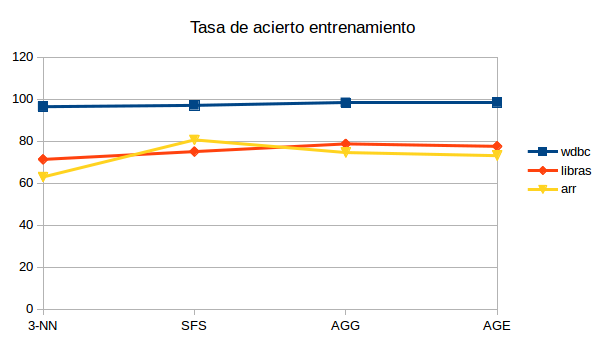
\includegraphics[width=130mm]{tasa_train_ag.png}
\end{figure}

Como podemos ver la tasa de acierto sobre Wdbc es la más elevada con respecto a las otras bases, además las tasas de acierto de todos lo algoritmos sobre esta base son muy parecidas, esto se debe a que, como dijo el profesor, esta base de datos es muy pequeña, es decir, el espacio de búsqueda es muy pequeño ($2^{30}$) y hay muy poca tasa de mejora entre una solución y otra.\\

Las tasas de acierto tanto para arritmia como para libras no difieren más que aproximadamente un 5\% para cada algoritmo. Es importante señalar cómo la tasa de acierto de los algoritmos usados en mejor que la tasa que da el 3NN original, es decir, usando todos los datos de la muestra. Con lo cual aquí se pone de manifiesto cómo el hecho de reducir el número de características a considerar no merma la correcta clasificación de los datos, al menos dentro de la muestra, ya veremos qué sucede fuera. De hecho reduciendo el número de características no sólo reducimos el cómputo necesario sino también el posible ruido que pueden tener algunos datos.\\

Es curioso ver cómo el algoritmo greedy produce los mejores resultados en la base de datos con un espacio de búsqueda mayor, de hecho produce mejores resultados en esa base de datos que en la de libras que tiene un espacio menor (es el único que lo hace), probablemente por la naturaleza de los datos, es decir, cómo de distintas sean las muestras que componen las distintas clases entre sí. En mi opinión el hecho de que el SFS produzca mejores resultados que la mayoría en el espacio de búsqueda más grande se debe a que al fin y al cabo el greedy en cada momento va construyendo la mejor solución que puede mientras que en cambio el resto de métodos depende más de cómo de buena sea la exploración que realicen.\\

En cambio sí podemos ver cómo para el espacio más reducido de libras (también se ve en wdbc) sí que los algoritmos que hacen una búsqueda más extensa en el terreno, los genéticos, dan resultados mejores que SFS ya que exploran más soluciones y por lo tanto tienen mayor posibilidad de encontrar una mejor.\\

Si ahora comparamos los dos algoritmos genéticos vemos como el AGG da mejores resultados en libras y en arritmia. En wdbc es el AGE el que obtiene un mejor resultado aunque con una diferencia más pequeña que la que tienen los dos algoritmos en las otras BBDD; ya hemos dicho que esta base de datos es muy pequeña y que hay poca variación de una solución a otra.\\

Vamos a ver unos datos que pueden ser interesantes para la comparación de ambos algoritmos y que han sido calculados de forma aproximada ya que sí bien para AGE siempre se realiza el mismo número de cruces y mutaciones por iteración y en consecuencia el mismo número de evaluaciones de la función objetivo, en AGE la mutación se da con una cierta probabilidad con lo que las cifras que hemos calculado son aproximadas:\\

\begin{table}[H]
\centering
\caption{Datos algoritmos genéticos}
\label{my-label}
\resizebox{\textwidth}{!}{\begin{tabular}{l|l|l|l|l|l|l|l|l|l|l|l|l|l|l|l|}
\cline{2-16}
                          & \multicolumn{5}{c|}{Wdbc}                                            & \multicolumn{5}{c|}{Movement\_Libras}                                & \multicolumn{5}{c|}{Arrhythmia}                                      \\ \cline{2-16} 
                          & n\_iters & cruces/iter & mutaciones/iter & n\_cruces & n\_mutaciones & n\_iters & cruces/iter & mutaciones/iter & n\_cruces & n\_mutaciones & n\_iters & cruces/iter & mutaciones/iter & n\_cruces & n\_mutaciones \\ \hline
\multicolumn{1}{|l|}{AGG} & 651      & 22          & 1               & 14322     & 651           & 599      & 22          & 3               & 13178     & 1797          & 483      & 22          & 9               & 10626     & 4347          \\ \hline
\multicolumn{1}{|l|}{AGE} & 7267     & 2           & 0.06            & 14534     & 436           & 6867     & 2           & 0.18            & 13734     & 1236          & 5871     & 2           & 0.55            & 11742     & 3228          \\ \hline
\end{tabular}}
\end{table}

Pese a que ambos algoritmos funcionan de un modo similar ya que ambos realizan un cruce de unos padres seleccionados y luego mutan sobre la población de hijos obtenidos en mi opinión el AGE es más conservador, quiero decir, los saltos que se producen de una generación a otra en el AGG son con mayor brusqueda ya que no solo cruzamos muchos más padres dando lugar a una mayor recombinación de genes por iteración sino que también ser realiza un mayor número de mutaciones por iteración. Con lo cual es mi opinión esto hace que el AGG sea un algoritmo con una componente de diversificación más fuerte que el AGE, lo que puede ser el motivo por el cual el AGG de mejores resultados en las bases de datos grandes (además del azar siempre presente en estos algoritmos).\\

Como vemos el AGE presenta un mayor número de cruces, pero un cruce siempre conserva más información de la población anterior que una mutación (pese a que en nuestro caso el número de mutaciones que se da en ambos algoritmos es bastante pequeño). Entonces el AGE no realiza una exploración tan amplia del espacio de soluciones.\\

\begin{figure}[H]
\centering
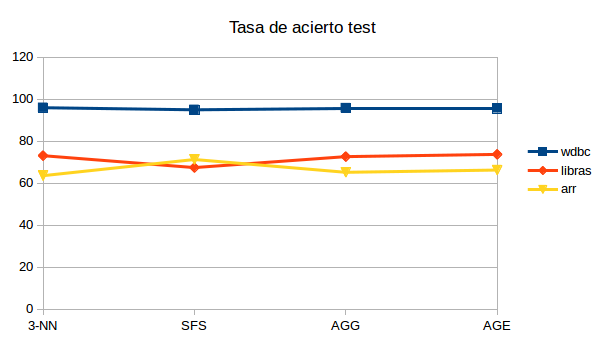
\includegraphics[width=130mm]{tasa_test_ag.png}
\end{figure}

Veamos ahora cómo se comportan los algoritmos con respecto a la clasificación que producen sus características seleccionadas para los datos fuera de la muestra de entrenamiento. Lo primero que señalamos es que en la amplia mayoría de los casos la tasa de acierto es mayor dentro de la muestra que fuera, pero hay algunos casos donde es al revés. Esto se debe a que es probable que haya muestras de entrenamiento de una clase más cercanas a otra muestra pese a no pertenecer a la clase de dicha muestra. Con lo cual se puede dar el caso de que la "votación" sea mala en la muestra y en cambio la muestra fuera la distribución de puntos sea más favorable a una correcta clasificación de los datos. Por lo tanto no tiene que extrañarnos demasiado esto. Quizás si usásemos un 1NN sí que sería más probable que la muestra más cercana a otra perteneciera a la misma clase que ella (decimos la más cercana y no que en el 1NN hubiésemos obtenido una tasa de acierto del 100\% dentro de la muestra puesto que usamos para evitar esto el Leave One Out).\\

Nuevamente el comportamiento para Wdbc es muy similar para todos los algoritmos, lo que era esperable por el razonamiento que hemos dado antes. Lo que sí podemos ver es cómo en esta ocasión el 3NN está en los primeros puestos para las bases de datos de wdbc y libras además de que hay otros algoritmos que también cambian de posición. Esto nos informa de dos cosas: la primera es del eterno problema que hay en el aprendizaje automático y es la capacidad de generalización, el no poder asegurar que si una solución es buena dentro de la muestra de entrenamiento vaya a ser fuera. En segundo lugar vemos cómo lo algoritmos son fuertemente dependientes de los datos, el ruido o simplemente los datos tomados afectan al rendimiento de las soluciones encontradas.\\

Esto último se pone muy en relieve cuando vemos cómo el GRASP es de los peores algoritmos en las bases de datos de wdbc y libras, en mi oponión se ve más afectada en estas bases porque puede ser que los datos tengan ruido o no informen lo suficiente y al ser el algoritmo que mayor intesificación realiza puede que sea el que más sufre de sobreajuste. Ahora bien, en la base de datos de arritmia es el mejor algoritmo indicando que o bien los datos de esta base dan mucha información o que el espacio de búsqueda queda grande para el resto de algoritmos que dependen más de la exploración realizada. De hecho el otro algoritmo que peor funciona en libras y wdbc es precisamente el SFS que también puede verse afectado por el sobreajuste al no tener mecanismos de diversificación.\\

El hecho de que el 3NN con toda la información no mejore a todos los algoritmos puede venir de que no sólo haya características irrelevantes sino que, como hemos señalado anteriormente, haya datos cuya medición haya sido errónea y que simplemente lo que nos estén haciendo sea empeorar el resultado.\\

\begin{figure}[H]
\centering
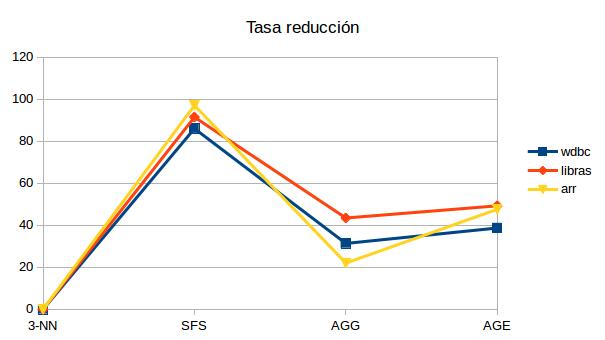
\includegraphics[width=130mm]{reduccion_ag.png}
\end{figure}

Evidentemente la tasa de reducción para el 3NN es 0 pues tomamos todas las características al no tener otro criterio. Ahora el que produce mayor reducción es el greedy lo que es lógico por la forma en la que trabaja, agregando progresivamente propiedades hasta no encontrar mejora ninguna.\\

Como era de esperar el siguiente que tiene una mayor tasa de reducción es el GRASP el cual al fin y al cabo tiene un comportamiento greedy y como las soluciones que produce el greedy aleatorio (que es el que genera mayor reducción) ya son los suficientemente buenas la búsqueda local no le "añade" muchas más características a la solución de la que parte.

Las tasas de reducción para el resto la BMB y el ILS son muy similares entre sí, si lo pensamos dado que nuestra función de coste sólo tiene en cuenta la tasa media de acierto en la muestra de entrenamiento (no tenemos en cuenta también la reducción que consigue) es lógico que esto suceda así, o al menos que no haya un algoritmo que claramente produzca mejores resultados que otro. La exploración que se hace es de algún modo u otro aleatoria con lo que dependiendo del azar será un algoritmo o el otro el que obtenga una solución con un menor número de características.\\


\begin{figure}[H]
\centering
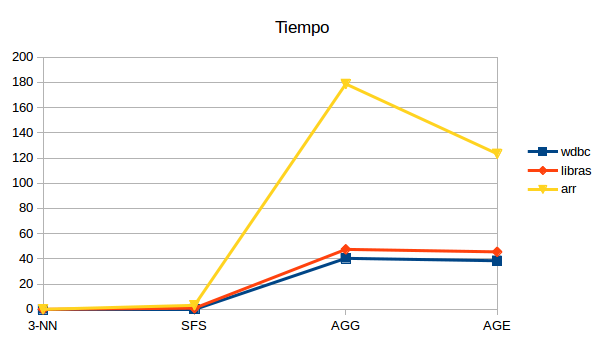
\includegraphics[width=130mm]{tiempo_ag.png}
\end{figure}


Evidentemente el 3NN tarda 0 segundo puesto que su tiempo de búsqueda de solución es 0 pues simplemente devuelve un solución con todos los valores a True, es decir, escoge todas las características sin tener ningún criterio. Y observamos también que todos los algoritmos si los analizamos individualmente tardan más cuanto mayor es el espacio de búsqueda (ahora el LOO no tiene tanto impacto y con lo cual el número de muestras por partición no resulta tan decisivo como sí ocurría en la práctica anterior cuando se tardaba más en libras que en arritmia para algunos algoritmos).\\

El GRASP es el algoritmo que tarda salvo en arritmia donde sólo le supero la BMB. Esto se debe a que es el que realiza las operaciones más costosas al hacer por cada ejecución un greedy y a continuación una búsqueda local. Sin embargo en la base de datos con un espacio de búsqueda mayor es la BMB la que más tarda, probablemente esto se deba a que pese a que la generación de la solución de la que parte la BL en GRASP es más costosa en tiempo sí que hace que se parta de una buena solución y que por tanto la BL tarde menos en no poder mejorar la solución de la que parte, algo que es muy importante cuando el espacio de búsqueda es tan grande.

De los tres algoritmos que hemos implementado en esta práctica el ILS es el más rápido esto se debe a la combinación de dos factores: las operaciones que realiza son poco costosas con respecto a las de los otros dos algoritmos y además tiene una componente de intesificación al mutar, un 10\% solamente, la mejor solución encontrada hasta el momento, haciendo, como hemos analizado anteriorment, que la BL tarde menos. De hecho vemos como en bases de datos con un espacio de búsqueda menor ILS y BMB tienen tiempos similares ya que esta intensificación no tiene tanta importancia.\\

Por último el SFS tarda muy poco con respecto al resto de algoritmos ya que se trata únicamente de una búsqueda greedy y no 25 como hace GRASP ni 25 búsquedas locales como hacen los otros algoritmos.\\

\newpage
\section{\color[rgb]{0.0,0.0,0.21}Bibliografía}

\begin{itemize}
\item Documentación del módulo scikit-learn: \url{http://scikit-learn.org/stable/documentation.html}
\item Documentación de Numpy: \url{http://docs.scipy.org/doc/}
\end{itemize}
\end{document}